\subsection{Infinite work-stealing deque}

\begin{tirPrefix}{inf-ws-deque-}

\subsubsection{Specification}

\begin{figure}
\begin{mathparpagebreakable}
    \iPersistent{(\inv\ t\ \iIname)}
  \\
    \infer[model-exclusive]{
        \model\ t\ \zooVals_1
      \\
        \model\ t\ \zooVals_2
    }{
      \iFalse
    }
  \and
    \infer[owner-exclusive]{
        \owner\ t\ \zooValsTwo_1
      \\
        \owner\ t\ \zooValsTwo_2
    }{
      \iFalse
    }
  \and
    \infer[owner-model]{
        \owner\ t\ \zooValsTwo
      \\
        \model\ t\ \zooVals
    }{
      \l{suffix}\ \zooVals\ \zooValsTwo
    }
  \\
    \iSpec[
      lab=create-spec
    ]{
      \iTrue
    }{
      \c{create}\ \c{()}
    }[
      t
    ]{
      \inv\ t\ \iIname \iSep \\
      \model\ t\ \nil \iSep \\
      \owner\ t\ \nil
    }
  \and
    \iAspec[
      lab=size-spec,
      mask=\iIname
    ]{
      \inv\ t\ \iIname \iSep \\
      \owner\ t\ \zooValsTwo
    }[
      \zooVals
    ]{
      \model\ t\ \zooVals
    }{
      \c{size}\ t
    }{
      \l{suffix}\ \zooVals\ \zooValsTwo \iSep \\
      \model\ t\ \zooVals
    }[
      \v{res}
    ]{
      \v{res} = \l{length}\ \zooVals \iSep \\
      \owner\ t\ \zooVals
    }
  \and
    \iAspec[
      lab=is-empty-spec,
      mask=\iIname
    ]{
      \inv\ t\ \iIname \iSep \\
      \owner\ t\ \zooValsTwo
    }[
      \zooVals
    ]{
      \model\ t\ \zooVals
    }{
      \c{is\_empty}\ t
    }{
      \l{suffix}\ \zooVals\ \zooValsTwo \iSep \\
      \model\ t\ \zooVals
    }[
      \v{res}
    ]{
      \v{res} = \decideEq{\zooVals}{\nil} \iSep \\
      \owner\ t\ \zooVals
    }
  \and
    \iAspec[
      lab=push-spec,
      mask=\iIname
    ]{
      \inv\ t\ \iIname \iSep \\
      \owner\ t\ \zooValsTwo
    }[
      \zooVals
    ]{
      \model\ t\ \zooVals
    }{
      \c{push}\ t\ \zooVal
    }{
      \l{suffix}\ \zooVals\ \zooValsTwo \iSep \\
      \model\ t\ (\zooVals \dplus [\zooVal])
    }[
      \c{()}
    ]{
      \owner\ t\ (\zooVals \dplus [\zooVal])
    }
  \and
    \iAspec[
      lab=steal-spec,
      mask=\iIname
    ]{
      \inv\ t\ \iIname
    }[
      \zooVals
    ]{
      \model\ t\ \zooVals
    }{
      \c{steal}\ t
    }{
      \model\ t\ (\l{tail}\ \zooVals)
    }[
      \v{res}
    ]{
      \v{res} = \l{head}\ \zooVals
    }
  \and
    \iAspec[
      lab=pop-spec,
      mask=\iIname
    ]{
      \inv\ t\ \iIname \iSep \\
      \owner\ t\ \zooValsTwo
    }[
      \zooVals
    ]{
      \model\ t\ \zooVals
    }{
      \c{pop}\ t
    }[
      o\ \zooValsTwo'
    ]{
      \l{suffix}\ \zooVals\ \zooValsTwo \iSep \\
      \matchOption{
        o
      }{
        \zooVals = \nil \iSep
        \zooValsTwo' = \nil \iSep \\
        \model\ t\ \nil
      }{
        \zooVal
      }{
        \Exists \zooVals'. \\
        \zooVals = \zooVals' \dplus [\zooVal] \iSep
        \zooValsTwo' = \zooVals' \iSep \\
        \model\ t\ \zooVals'
      }
    }[
      \v{res}
    ]{
      \v{res} = o \iSep \\
      \owner\ t\ \zooValsTwo'
    }
\end{mathparpagebreakable}
\caption{\ocamlinline{Inf_ws_deque}: Specification}
\label{fig:chaselev_inf_ws_deque_spec}
\end{figure}


The specification of the infinite-array-based version is given in \cref{fig:chaselev_inf_ws_deque_spec}.
It features three predicates: \inv, \model and \owner.

The persistent assertion $\inv\ t$ represents the knowledge that $t$ is a valid deque.
It is returned by \c{create} (\refTirName{create-spec}) and required by all operations.

The exclusive assertion $\model\ t\ \zooVals$ represents the ownership of the content of the deque \zooVals.
It it returned by \c{create} and accessed atomically by all operations.

The exclusive assertion $\owner\ t\ \zooValsTwo$ represents the owner of the deque; \zooValsTwo is an upper bound on the current content of the deque (\refTirName{owner-model}).
It is returned by \c{create} and used by all private operation: \c{size} (\refTirName{size-spec}), \c{is\_empty} (\refTirName{is-empty-spec}), \c{push} (\refTirName{push-spec}) and \c{pop} (\refTirName{pop-spec}).
The only public operation is \c{steal} (\refTirName{steal-spec}), which does not require \owner.

Note that the public postconditions of the private operations are quite verbose.
This is due to the fact that \owner is passed to the operation and therefore cannot be combined with \model through \refTirName{owner-model} to get information about the content of the deque; instead, we provide such information in the public postcondition.
We need this expressivity in practice to verify a wrapper~\refLibTheoriesFile{zoo_saturn/inf_ws_deque_2} with better liveness properties.

\subsubsection{Weak specification.}

\begin{tirPrefix}{ws-deque-}

\begin{figure}
\begin{mathpar}
%    \iPersistent{(\inv\ t)}
%  \\
%    \iSpec[
%      lab=create-spec-weak
%    ]{
%      \iTrue
%    }{
%      \c{create}\ \c{()}
%    }[
%      t
%    ]{
%      \inv\ t \iSep \\
%      \model\ t\ \nil \iSep \\
%      \owner\ t
%    }
%  \and
%    \iAspec[
%      lab=push-spec-weak
%    ]{
%      \inv\ t \iSep \\
%      \owner\ t
%    }[
%      \zooVals
%    ]{
%      \model\ t\ \zooVals
%    }{
%      \c{push}\ t\ \zooVal
%    }{
%      \model\ t\ (\zooVals \dplus [\zooVal])
%    }[
%      \c{()}
%    ]{
%      \owner\ t
%    }
%  \and
    \iAspec[
      lab=steal-spec-weak
    ]{
      \inv\ t
    }[
      \zooVals
    ]{
      \model\ t\ \zooVals
    }{
      \c{steal}\ t
    }[
      o
    ]{
      \matchOption{
        o
      }{
        \model\ t\ \zooVals
      }{
        \zooVal
      }{
        \Exists \zooVals'. \\
        \zooVals = \cons{\zooVal}{\zooVals'} \iSep \\
        \model\ t\ \zooVals'
      }
    }[
      \v{res}
    ]{
      \v{res} = o
    }
  \and
    \iAspec[
      lab=pop-spec-weak
    ]{
      \inv\ t \iSep \\
      \owner\ t
    }[
      \zooVals
    ]{
      \model\ t\ \zooVals
    }{
      \c{pop}\ t
    }[
      o
    ]{
      \matchOption{
        o
      }{
        \model\ t\ \zooVals
      }{
        \zooVal
      }{
        \Exists \zooVals'. \\
        \zooVals = \zooVals' \dplus [\zooVal] \iSep \\
        \model\ t\ \zooVals'
      }
    }[
      \v{res}
    ]{
      \v{res} = o \iSep \\
      \owner\ t
    }
\end{mathpar}
\caption{\ocamlinline{Ws_deque}: Weak specification (excerpt)}
\label{fig:chaselev_ws_deque_spec_weak}
\end{figure}


\Citet{DBLP:journals/pacmpl/JungLCKPK23}%
\footnote{
See also the master thesis of \citet{DBLP:journals/corr/abs-2309-03642}.
}
also worked on the verification of the Chase-Lev work-stealing deque.
However, we argue that the specification they prove, given in \cref{fig:chaselev_ws_deque_spec_weak}, is unsatisfactory.
Indeed, contrary to our specification, \refTirName{steal-spec-weak} and \refTirName{pop-spec-weak} say nothing about the observed content of the deque when the operation fails.

In practice, these weaker specifications, especially that of \c{pop}, are not sufficient to reason about the \emph{termination} of a work-stealing scheduler.
In \cref{sec:parabs}, we show how our strong specifications are lifted all the way up to the scheduler.

Another point we would like to make is that weakening the specification does make the verification simpler, but one may argue that the most subtle and interesting part of it is lost.

\end{tirPrefix}

\subsubsection{Implementation}

\begin{figure}
\centering
\scalebox{.8}{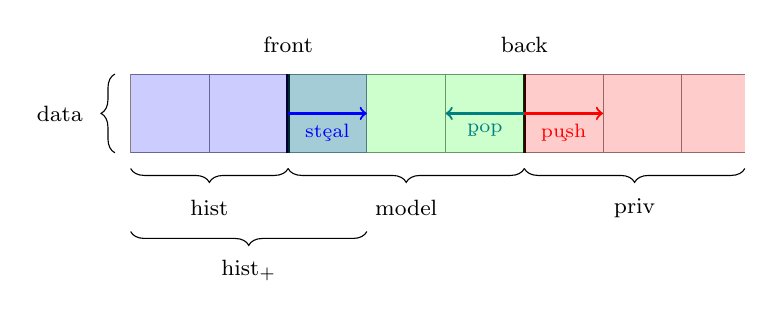
\begin{tikzpicture}
  \def\hist{2}
  \def\histx{1}
  \def\model{3}
  \def\priv{2.8}

  \draw[step=1cm, gray] (0, 0) grid ++(\hist + \model + \priv, 1) ;
  \draw[decorate, decoration={brace, amplitude=5pt}] (-0.2, 0) -- ++(0, 1) node [midway, xshift=-7mm] {\footnotesize data} ;

  \draw[very thick] (\hist, 0) -- ++(0, 1) node[label=above:\footnotesize front] {} ;

  \draw[very thick] (\hist + \model, 0) -- ++(0, 1) node[label=above:\footnotesize back] {} ;

  \fill[red, opacity=0.2] (\hist + \model, 0) rectangle ++(\priv, 1) ;
  \draw[decorate, decoration={brace, amplitude=5pt}] (\hist + \model + \priv, -0.2) -- ++(- \priv, 0) node [midway, yshift=-5mm] {\footnotesize priv} ;

  \fill[green, opacity=0.2] (\hist, 0) rectangle ++(\model, 1) ;
  \draw[decorate, decoration={brace, amplitude=5pt}] (\hist + \model, -0.2) -- ++(- \model, 0) node [midway, yshift=-5mm] {\footnotesize model} ;
  \fill[blue, opacity=0.2] (0, 0) rectangle ++(\hist, 1) ;
  \draw[decorate, decoration={brace, amplitude=5pt}] (\hist, -0.2) -- ++(- \hist, 0) node [midway, yshift=-5mm] {\footnotesize hist} ;

  \fill[blue, opacity=0.2] (\hist, 0) rectangle ++(\histx, 1) ;
  \draw[decorate, decoration={brace, amplitude=5pt}] (\hist + \histx, - 1) -- ++(- \hist - \histx, 0) node [midway, yshift=-5mm] {\footnotesize hist\textsubscript{+}} ;

  \draw[thick, ->, blue] (\hist, 0.5) -- ++(1, 0) node[midway, below] {\scriptsize\c{steal}} ;

  \draw[thick, ->, teal] (\hist + \model, 0.5) -- ++(- 1, 0) node[midway, below] {\scriptsize\c{pop}} ;
  \draw[thick, ->, red] (\hist + \model, 0.5) -- ++(1, 0) node[midway, below] {\scriptsize\c{push}} ;
\end{tikzpicture}}
\caption{\ocamlinline{Inf_ws_deque}: Physical state}
\label{fig:chaselev_inf_ws_deque_physical_state}
\end{figure}


The implementation relies on
(1) an infinite array,
(2) a \emph{monotonic} front index for the thieves, and
(3) a back index reserved for the owner of the deque.

In general, we can divide the infinite array as in \cref{fig:chaselev_inf_ws_deque_physical_state}.
The first part, between 0 and the front index, corresponds to the \emph{persistent} history of stolen values.
The second part, between the two indices, corresponds to the logical content of the deque, as represented by \model.
The last part, beyond the back index, corresponds to the private section of the array, reserved for the owner.

Given this representation, the algorithm proceeds as follows.
$\c{push}\ t\ \zooVal$ writes \zooVal into the first private cell and atomically increments the back index, thereby publishing the value.
Symmetrically, $\c{pop}\ t$ atomically decrements the back index and returns the value of the cell it just privatized.
$\c{steal}\ t$ is much more careful:
(1) it reads the front and the back indices;
(2) if the deque looks empty, it fails;
(3) otherwise, it attempts to advance the front index;
(4) if the update succeeds, the value at the front index is returned;
(5) otherwise, it starts over.

The above description overlooked one crucial aspect: what happens at the limit, when \c{pop} and \c{steal} compete for the last value in the deque?
In that case, the deque must be \emph{stabilized}: \c{pop} also attempts to advance the front index before incrementing the back index --- whether it wins the update or not --- thereby equalizing the two indices.

\subsubsection{Logical states}

\begin{figure}
\centering
\scalebox{.8}{\begin{tikzpicture}
  \def\width{4cm}
  \def\height{2cm}

  \node[align=center] (s1) {
    \ding{172} empty \\
  	\begin{tikzpicture}[scale=0.5]
      \def\hist{2}
      \def\priv{2.8}

      \draw[step=1cm, gray] (0, 0) grid (\hist + \priv, 1) ;

      \fill[blue, opacity=0.2] (0, 0) rectangle (\hist, 1) ;
      \draw[very thick] (\hist, 1) -- ++(0, - 1) node[yshift=2mm, label=below:{\tiny front = back}] {} ;
      \fill[red, opacity=0.2] (\hist, 0) rectangle ++(\priv, 1) ;
    \end{tikzpicture}
  } ;

  \node[align=center] (s2) [right=\width of s1] {
    \ding{173} non-empty \\
    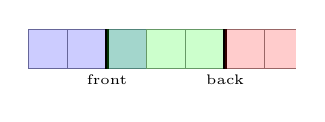
\begin{tikzpicture}[scale=0.5]
      \def\hist{2}
      \def\histx{1}
      \def\model{3}
      \def\priv{1.8}

      \draw[step=1cm, gray] (0, 0) grid (\hist + \model + \priv, 1) ;

      \fill[blue, opacity=0.2] (0, 0) rectangle (\hist + \histx, 1) ;
      \draw[very thick] (\hist, 1) -- ++(0, - 1) node[yshift=2mm, label=below:{\tiny front}] {} ;
      \fill[green, opacity=0.2] (\hist, 0) rectangle ++(\model, 1) ;
      \draw[very thick] (\hist + \model, 1) -- ++(0, - 1) node[yshift=2mm, label=below:{\tiny back}] {} ;
      \fill[red, opacity=0.2] (\hist + \model, 0) rectangle ++(\priv, 1) ;
    \end{tikzpicture}
  } ;

  \node[align=center] (s3) [below=\height of s2] {
    \ding{174} emptyish \\
    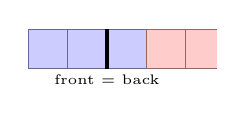
\begin{tikzpicture}[scale=0.5]
      \def\hist{2}
      \def\histx{1}
      \def\priv{2.8}

      \draw[step=1cm, gray] (0, 0) grid (\hist + \priv, 1) ;

      \fill[blue, opacity=0.2] (0, 0) rectangle (\hist + \histx, 1) ;
      \draw[very thick] (\hist, 1) -- ++(0, - 1) node[yshift=2mm, label=below:{\tiny front = back}] {} ;
      \fill[red, opacity=0.2] (\hist + \histx, 0) rectangle ++(\priv - \histx, 1) ;
    \end{tikzpicture}
  } ;
  \node[align=center] (s4) [below=\height of s1] {
    \ding{175} super-empty \\
    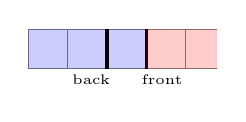
\begin{tikzpicture}[scale=0.5]
      \def\hist{2}
      \def\histx{1}
      \def\priv{2.8}

      \draw[step=1cm, gray] (0, 0) grid (\hist + \priv, 1) ;

      \fill[blue, opacity=0.2] (0, 0) rectangle (\hist + \histx, 1) ;
      \draw[very thick] (\hist, 1) -- ++(0, - 1) node[xshift=-2mm, yshift=2mm, label=below:{\tiny back}] {} ;
      \draw[very thick] (\hist + \histx, 1) -- ++(0, - 1) node[xshift=2mm, yshift=2mm, label=below:{\tiny front}] {} ;
      \fill[red, opacity=0.2] (\hist + \histx, 0) rectangle ++(\priv - \histx, 1) ;
    \end{tikzpicture}
  } ;

  \draw[thick, ->] (s1) to[bend left] node[above] {\c{push}} (s2) ;
  \draw[thick, ->] (s2) to[bend left] node[below] {\c{steal}} (s1) ;
  \draw[thick, ->] (s2) to[looseness=3, out=135, in=45] node[above] {\c{push}, \c{pop}, \c{steal}} (s2) ;
  \draw[thick, ->] (s2) to[bend left] node[right] {\c{pop}} (s3) ;
  \draw[thick, dotted, ->] (s3) to[bend left] node[below] {\c{pop}, \c{steal}} (s4) ;
  \draw[thick, dotted, ->] (s4) to[bend left] node[left] {\c{pop}} (s1) ;
  \draw[thick, ->] (s1) to[bend left] node[right] {\c{pop}} (s4) ;
  \draw[thick, dotted, ->] ([xshift=2mm]s1.south) to[bend left] ([xshift=2mm]s4.north) ;

  \matrix [right, nodes={font=\tiny}] at (current bounding box.south west) {
    \draw[thick, ->] (0, 0) -- (1em, 0) node[right] {linearization} ; \\
    \draw[thick, dotted, ->] (0, 0) -- (1em, 0) node[right] {stabilization} ; \\
  } ;
\end{tikzpicture}}
\caption{\ocamlinline{Inf_ws_deque}: Logical state}
\label{fig:chaselev_inf_ws_deque_logical_state}
\end{figure}


\Cref{fig:chaselev_inf_ws_deque_logical_state} tells the same story as above in terms of four \emph{logical states}:
(1) in the stable ``empty'' state, the deque is indeed empty, as indicated by the two equal indices;
(2) in the stable ``non-empty'' state, the \model is non-empty, meaning thieves may compete for the first value;
(3) in the unstable ``emptyish'' state, the thieves and the owner compete for the same value;
(4) in the unstable ``super-empty'' state, some operation won the value and the deque is waiting to be stabilized by the owner.

Let us now focus on the ``emptyish'' state.
In this physical configuration, it makes sense to say that the \model of the deque should be empty.
In fact, is has to be empty: if a \c{steal} operation observed this state, it would conclude that the deque is empty --- except under a weak specification.
But then, if the \model should be empty, which operation was linearized during the transition to the ``emptyish'' state?
We have no choice: it should be the winner of the front update, \ie the operation which triggers the transition to the ``super-empty'' state.
In conclusion, we have to predict the winner at each index using a multiplexed prophecy variable (see \cref{sec:prophecy}).

\end{tirPrefix}
